\begin{frame}{Crystal truncation rods}
    \begin{columns}
        
    \column[T]{0.34\textwidth}
    \small{
    \begin{table}
        \centering
        \begin{tabular}{ |l|l|l|l| }
            \hline
            Argon & \ammonia & \dioxygen & Duration \\
             & & & (hours) \\ 
            \hline
            50 & 0 & 0 & 24 \\
            42 & 0 & 8 & 12 \\
            41 & 1 & 8 & 5 \\
            \hline
            \rowcolor{lightblue}
            50 & 0 & 0 & 7 \\
            \rowcolor{lightorange}
            42 & 0 & 8 & 1 \\
            \rowcolor{lightgreen}
            41 & 1 & 8 & 10 \\
            \rowcolor{lightred}
            48.5 & 1 & 0.5 & 13 \\
            \rowcolor{lightgray}
            49 & 1 & 0 & 11 \\
            \rowcolor{lightbrown}
            50 & 0 & 0 & 8 \\
            \hline
            50 & 0 & 0 & 8 \\
            \rowcolor{lightpink}
            49.5 & 0 & 0.5 & 4 \\
            \hline
        \end{tabular}
        \caption{Gas flow in reactor ($50$ mL/min, $0.3$ bar). In experimental order.}
    \end{table}
    }
    
    \column[T]{0.6\textwidth}
    
        \begin{figure}
            \centering
            \begin{tikzpicture}
                \node (image) [anchor=south west, inner sep=0pt] {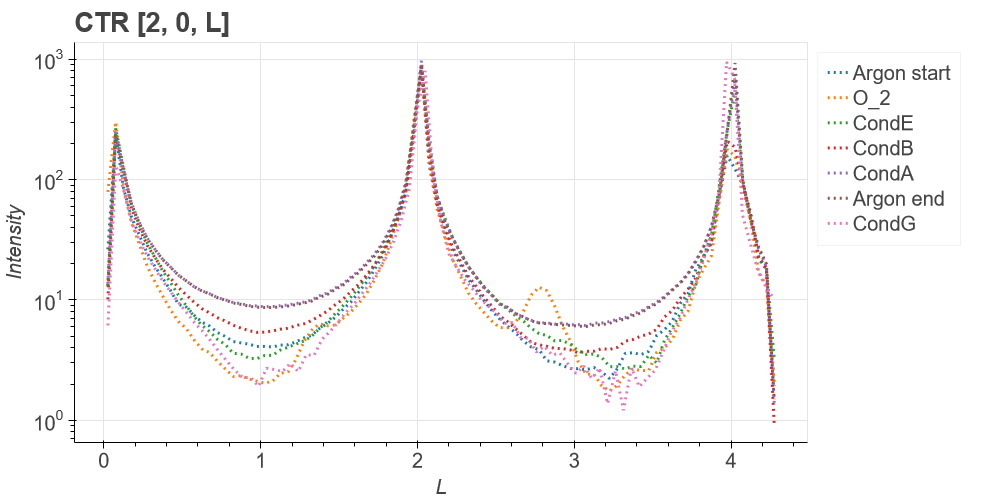
\includegraphics[width=0.98\textwidth, trim={0 0 8cm 0}, clip]{Figures/sxrd_data/ctr/CTR_2_0.png}};

                \begin{scope}[x={(image.south east)}, y={(image.north west)}]
                    \node [fill=white,rounded corners=2pt,inner sep=1pt] at (0.75,0.5) {\footnotesize \textcolor{orange}{Pt3O4 ($\approx$ 5 ML)}};
                    \node [fill=white,rounded corners=2pt,inner sep=1pt] at (0.35,0.7) {\footnotesize \dioxygen : roughness $\uparrow$};
                    \node [fill=white,rounded corners=2pt,inner sep=1pt] at (0.35,0.6) {\footnotesize \ammonia : roughness $\downarrow$};
                \end{scope}
                
            \end{tikzpicture}

            \caption{Crystal Truncation Rods (CTR) perpendicular to [2, 0] reciprocal space node.}
            \label{fig:CTR_2_0}
        \end{figure}
    
    \end{columns}

    \pause
    We can see the effect of the different atmospheres on the surface roughness.\\
    \pause
    There is a slight effect on the surface relaxation during reaction conditions that could also be a feature linked to Pt$_3$O$_4$ residues.
\end{frame}